\documentclass[english]{beamer}
\mode<presentation>

%\usepackage[slovak]{babel}
\usepackage[utf8]{inputenc}
\usepackage{physics}
\usepackage{tikz, pgfplots}
%\DeclareMathSizes{12pt}{10pt}{10pt}{10pt}

\usepackage{multimedia}
\RequirePackage{environ}

\usepackage{changepage}
\makeatletter
\newenvironment{forcecenter}%
    {\@parboxrestore%
     \begin{adjustwidth}{}{\leftmargin}%
    }{\end{adjustwidth}
     }
\makeatother

%\graphicspath{images}

%Use Okular!

\newcommand\Wider[2][3em]{
\makebox{\linewidth][c]{
	\begin{minipage}{\dimexpr\textwidth+#1\relax}
	\raggedright#2
	\end{minipage}	
	}
}
}

\NewEnviron{sea}{
	\fontsize{9}{12}
    \begin{eqnarray*}
   % \fontsize{12pt}{10pt}\selectfont
    \BODY
    \end{eqnarray*}
    \normalsize
}

\begin{document}

  \title{Simulation of boson dynamics: A coherent-states-based method}
  \author[Michal Horanský]{Michal Horanský\\\hfill\\University of Leeds}
  %\date{14. apríl 2019}
  %\maketitle
  \date{January 31, 2025}
  \begin{frame}
    \titlepage
  \end{frame}
    %\begin{center}
    %\includegraphics<1->[scale=0.5]{images/multipendulum_scheme.png}
    %\end{center}
  
  
  \begin{frame}
  	\frametitle{Introduction}
  	\framesubtitle{Curse of dimensionality}
  	\begin{itemize}
  		\item A system governed by a Hamiltonian $\hat{H}$ which preserves the total particle number $S$ across all $M$ modes.
  		\item We wish to find the time evolution of some quantum state $\ket{\Psi}$.
  		\item The Hilbert space is spanned by an occupancy number basis of dimension
  		$$\dim(\mathcal{H})={S+M-1\choose M-1}$$
  		which grows exponentially with $M$.
  	\end{itemize}
  \end{frame}
  
  \begin{frame}
  	\frametitle{Introduction}
  	\framesubtitle{Coherent states: construction}
  	\begin{itemize}
  		\item Since $H$ preserves $S$, its second quantization depends only on the dynamical operators $\hat{a}_i^\dag \hat{a}_j$, which form the Lie algebra for the dynamical group $G=SU(M)\otimes U(1)$.
  		\item $\mathcal{H}$ is spanned by the elements of $G$ acting on some reference state $\ket{\Psi_0}$, here chosen to be $\ket{0,\dots 0, S}$--hence $\hat{g}\ket{\Psi_0}$ forms a basis to $\mathcal{H}$.
  		\item There exists a stability subgroup $S \subset G$ which leaves $\ket{\Psi_0}$ invariant up to a constant factor.
  		\item Hence a suitable (over-)complete basis is given by the unnormalized states $\unnormket{z}=\exp\left[iz^i\hat{q}_i\right]\ket{\Psi_0}$, where $\hat{q}_i$ is an element of the Lie algebra of the quotient group $G/S$.
  		\item This is one way of constructing $SU(M)$ coherent states.
  	\end{itemize}
  \end{frame}
  
  
  
  \begin{frame}
  	\frametitle{Introduction}
  	\framesubtitle{Coherent states: utility}
  	\begin{itemize}
  		\item Coherent states evolve in a way that captures the dynamics of the Hamiltonian.
  		\item For this reason, a small sample of coherent states should form a suitable basis for the propagation of $\ket{\Psi}$ (especially if the initial value of $\ket{\Psi}$ is highly localized in $\unnormket{z}$).
  		\item Due to their structure, matrix elements of second-quantized Hamiltonians are easy to calculate in a coherent state basis.
  		\item I chose to construct the states unnormalized, so that $\unnormket{z}$ has no explicit dependence on $\pdv{z^*_i}$, allowing the use of Wirtinger calculus for the equations of motion.
  		\item Even if the basis states are unnormalized, $\ket{\Psi (t)}$ remains normalized if we set the initial decomposition coefficients so that $\braket{\Psi(t=0)}{\Psi(t=0)}=1$
  	\end{itemize}
  	
  	%\begin{figure}
	%\centering
    		%\includegraphics[width=0.9\textwidth]{images/QD_schematic}
    		%\caption{Gross spectrum of a $C_{3v}$ InGaAs QD. Image credit: Karlsson, K. F. et al (2015), Spectral signatures of high-symmetry quantum dots and effects of symmetry breaking. New Journal of Physics, 17 103017}
    		%\label{fig:qd}
	%\end{figure}
  \end{frame}
  
  \begin{frame}
  	\frametitle{Results so far}
  	\framesubtitle{Two applications}
  	\begin{itemize}
  		\item I tried to reproduce two papers studying $SU(M)$ Hamiltonians:
  		\begin{itemize}
  			\item Qiao and Grossmann's paper on the Bose-Hubbard model
  			\item Green and Shalashilin's paper on bosons in a displaced harmonic trap
  		\end{itemize}
  		\item For each of these Hamiltonians, I have simulated the time-evolution of an initially pure coherent state $\unnormket{z_0}$ in two ways:
  		\begin{enumerate}
  			\item Uncoupled basis: Each basis state is propagated separately ($\dim = M-1$), then the decomposition coefficients are propagated on top of the evolved basis ($\dim = N$).
  			\item Variational method: The basis states and decomposition coefficients are fully coupled and propagated simultaneously ($\dim = N\cdot M$).
		\end{enumerate}	 
  	\end{itemize}
  \end{frame}
  
  \begin{frame}
  	\frametitle{Results so far}
  	\framesubtitle{Bose-Hubbard model}
  	\begin{figure}
	\centering
    		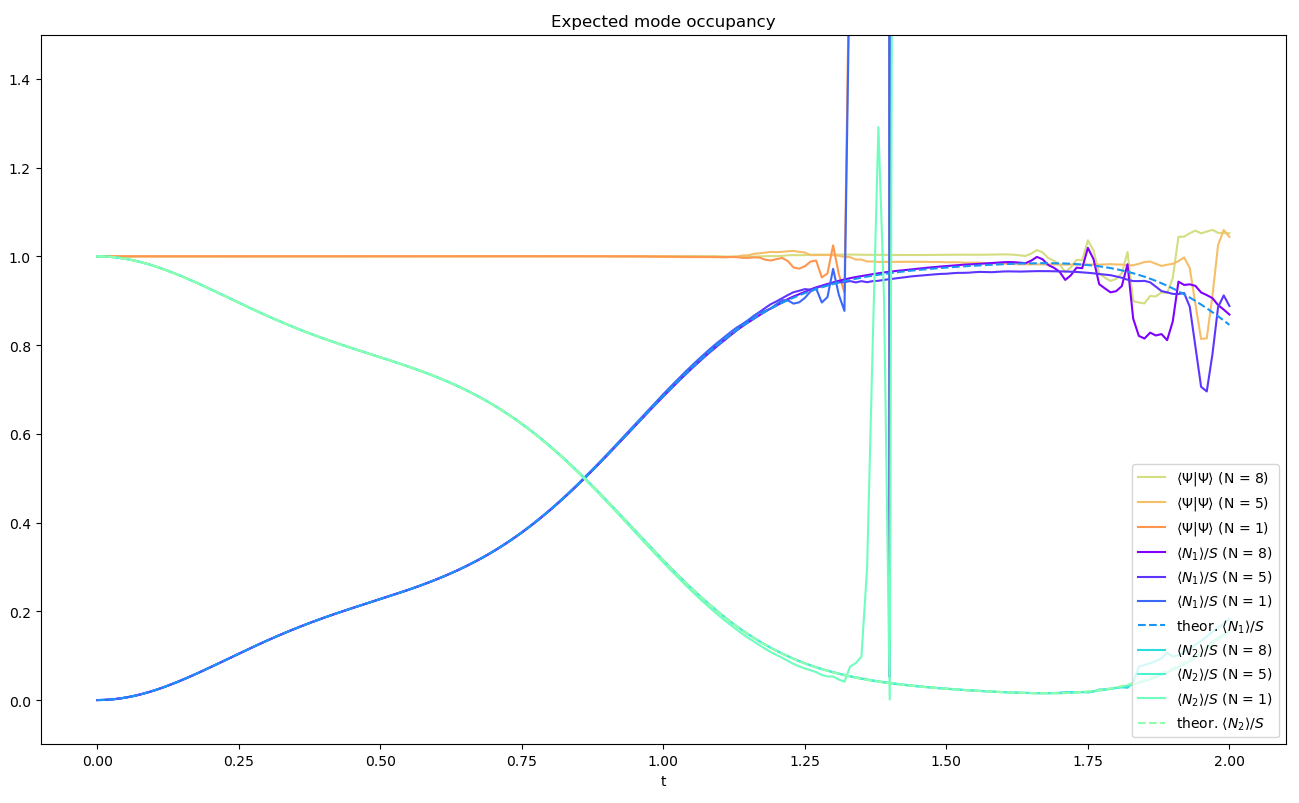
\includegraphics[width=0.9\textwidth]{images/BH_M=2}
    		\caption{$M=2, S=10, \ket{\Psi(t=0)}=n\unnormket{0.0+0.0i}$. $J(t)=1+\frac{1}{2}\cos(2\pi t), U=0.1, K=0$}
    		\label{fig:BH2}
	\end{figure}
  \end{frame}
  
  \begin{frame}
  	\frametitle{Results so far}
  	\framesubtitle{Bose-Hubbard model}
  	\begin{figure}
	\centering
    		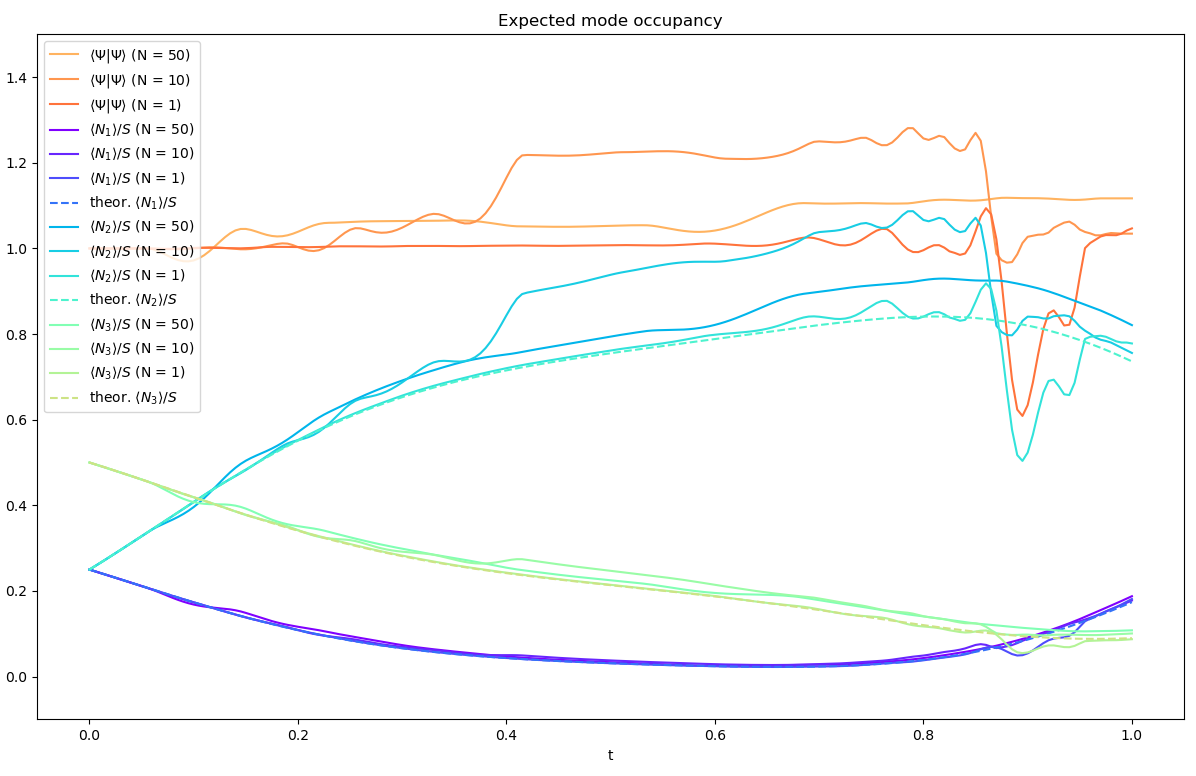
\includegraphics[width=0.9\textwidth]{images/BH_M=3}
    		\caption{$M=3, S=10, \ket{\Psi(t=0)}=n\unnormket{0.5+0.5i,0.5-0.5i}$. $J(t)=1+\frac{1}{2}\cos(2\pi t), U=0.1, K=0$}
    		\label{fig:BH3}
	\end{figure}
  \end{frame}
  
  \begin{frame}
  	\frametitle{Results so far}
  	\framesubtitle{Displaced harmonic trap}
  	\begin{figure}
	\centering
    		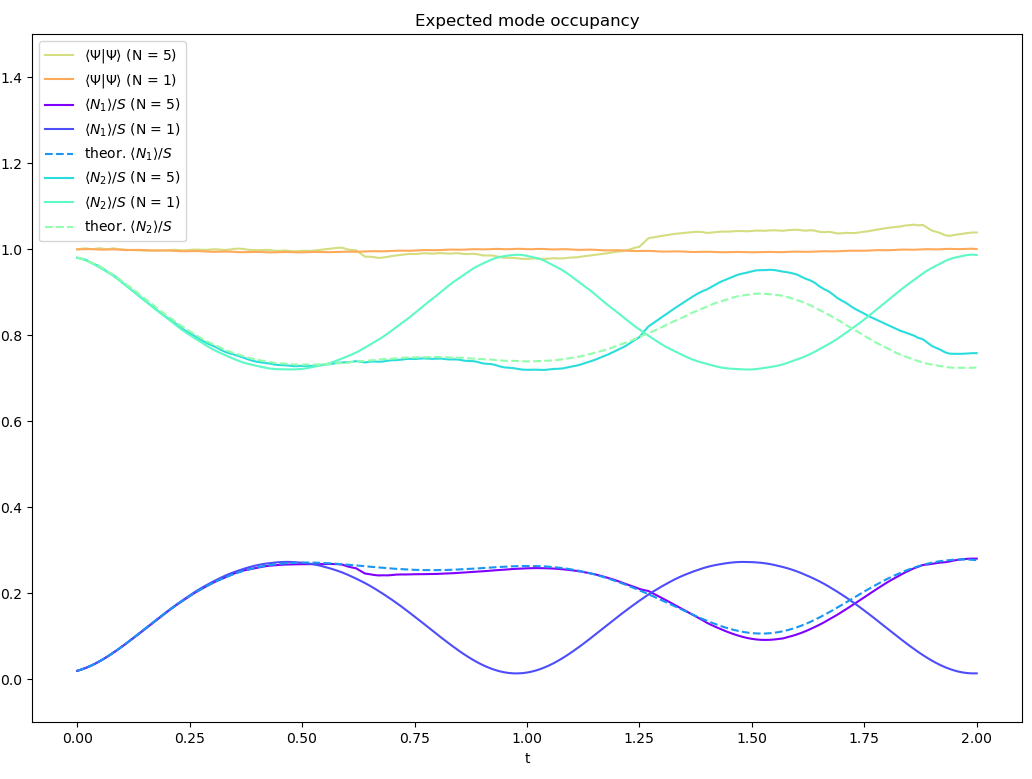
\includegraphics[width=0.9\textwidth]{images/DHT_M=2}
    		\caption{$M=2, S=10, \ket{\Psi(t=0)}=n\unnormket{0.1+0.1i}$. $\xi=2.1, \lambda_0=0.01$}
    		\label{fig:DHT2}
	\end{figure}
  \end{frame}
  
  \begin{frame}
  	\frametitle{Results so far}
  	\framesubtitle{Displaced harmonic trap}
  	\begin{figure}
	\centering
    		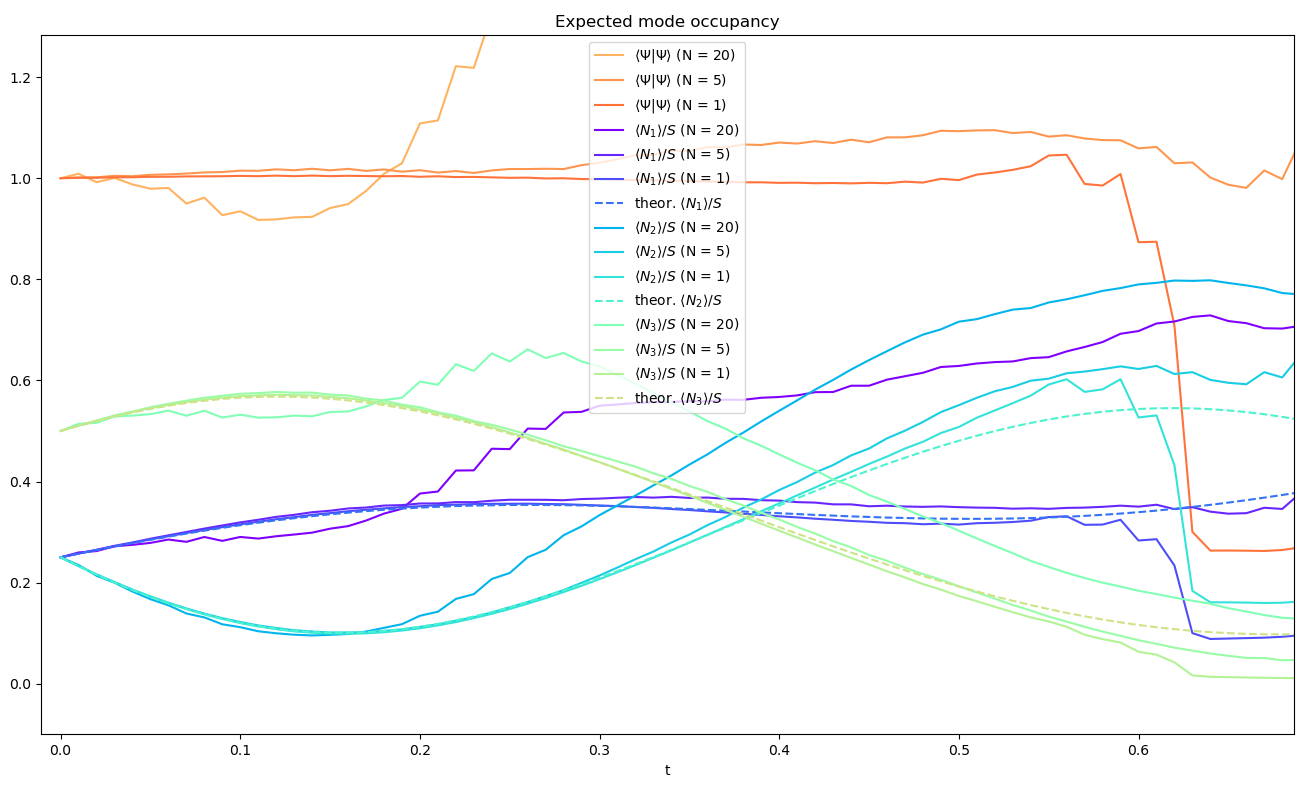
\includegraphics[width=0.9\textwidth]{images/DHT_M=3}
    		\caption{$M=3, S=10, \ket{\Psi(t=0)}=n\unnormket{0.5+0.5i,0.5-0.5i}$. $\xi=2.1, \lambda_0=0.01$}
    		\label{fig:DHT3}
	\end{figure}
  \end{frame}
  
  \begin{frame}
  	\frametitle{Outlook}
  	\begin{itemize}
  		\item Much faster (DHT with $M=3$: 1.5 minutes for an $N=20$ basis vs. 25 minutes for the occupancy basis solution)
  		\item Numerically unstable (big $M$, big $S$, conditioning, regularisation...)
  		\item Systems with different dynamical groups?
  	\end{itemize}
  \end{frame}
  
  \begin{frame}[plain,c]
  	\begin{center}
  	  \Huge Thank you for your attention
  	\end{center}
  \end{frame}


\end{document}